\begin{abstract}
我们研究双黑洞群体中的哪些指定比较，能够经受后验表示、选择银行表示和有限数值积分的变化。对固定的\DataEvents{}个公开事件，恢复了分析来源和原始先验后验，共\DataRows{}行。每事件选择一套Phenom族分析，不假设全目录配置完全相同。我们分别传播六个原生倾角模型和六个负有效自旋控制模型。后者的双星总体比例$g=P(\ceff<0)$在匹配滤波口径下的中位数为13.29\%至28.66\%，各模型90\%可信区间明显重叠。同一角度形状下，改变自旋幅度族使中位数相差12.10--14.34个百分点。这三项差异在\DataReplicates{}次成对人工事件/注入抽稀中均为正，而接近零的一项原生倾角差会变号。我们进一步将这种有限银行稳定性与缺失支持不确定性分开：声明的单事件积分补入族，在极限情形下可使部分$g$中位数移动最多\DataCompletionMax{}个百分点，但样本并未测出补入量。我们推导未知对数似然修正有界时的条件后验包络，并量化幅度排序的充分保证何时失效。仅凭检出概率上界，无法认证O3已知支持外贡献可忽略。这些结果构成可复查的条件研究与数值验证，不是天体物理形成渠道比例测量，也不是实际活动覆盖率校准。
\end{abstract}
\noindent\textbf{关键词：}引力波；双黑洞；群体推断；选择效应；重要性抽样；可复现研究。

\section{科学问题与既有研究}
不同黑洞形成途径可能预言不同的质量、自旋、红移及其相关性。推断渠道分支比例，需要物理群体预言和一致的观测似然。偏好对齐的现象学分量不对应唯一形成标签。已有多物理渠道研究明确说明，遗漏渠道和不确定物理设定会影响这些解释\cite{zevin}。

倾角分布对模型族和先验的敏感性已有直接研究\cite{spinlike}；共同自旋参考定义也是既有必要条件\cite{infinity}，并非本项目的新提议。层次重要性抽样中的数值不确定性已有系统讨论\cite{growing}，其中也包括注入银行及其抽稀对照\cite{structure}。现代注入使用说明明确要求提议分布覆盖目标支持\cite{injections}。我们不将这些原则、积分型自旋指标或重采样本身视为新方法。

较新的工作推荐积分型角度比例，同时表明大型模拟目录仍可能出现误导性的倾角结构\cite{longroad}。有效自旋几何与分量自旋建模假设也可以复现表观方向特征\cite{degeneracies}。事件层自旋先验选择会影响数值收敛和模拟群体恢复\cite{spinpriors}。本研究归一化的符号/形状控制没有消除这些歧义。我们没有实现这些研究的完整模型，也不声称独立发现先验敏感性；这些问题与本稿结果的解释直接重合。

本课题最初关注形成渠道解释对模型假设和选择效应是否稳健。目前证据支持这一问题中的必要基础层：哪些明确指定的群体比较，在恢复源数组并扰动数值银行后仍然存在；哪些贡献仅凭银行仍无法识别。这不能替代最终的物理渠道对照。本稿具体提供来源连接、可复现的条件差异、参考依赖派生字段不一致的实例，以及已有银行波动与未见贡献假设之间的定量区分。这些具体实例的独立新颖性尚未确认。

本稿扩展了项目v0.2论文的数值范围，同时保留旧版本及其冻结产物。这是一份阶段性研究稿：实际遗漏似然界、共同参考下的倾角群体分析和历史注入执行信息仍未完成。缺少这些环节，不能算作成功测出了形成渠道比例。

\section{数据与分析来源}\label{sec:data}
\subsection{固定事件集合与完整来源恢复}
研究起点是GWPopulation的GWTC-3教程\cite{tutorial}。教程数组适合作为历史基线，不是官方群体分析的唯一表示。本项目按记录的搜索显著性和伴星质量条件保留固定\DataEvents{}事件。十项初始缺失FAR已追溯到目录合并时的覆盖，并以早期搜索记录核查；没有事件仅因FAR缺失而被默认为通过。事件数相同，不能证明与另一研究的成员、分类规则或波形选择一致。

我们从固定GWTC-2.1和GWTC-3记录恢复原始先验发布文件\cite{pe21,pe3}。69份文件共\DataBytes{}字节，官方MD5与本地SHA-256均已核验。得到的\DataRows{}行保留源坐标、自旋方位角及可用派生字段。分析来源由逐行连接、配置和先验信息确定；包含这些行的容器标签不一定唯一。一项歧义分析通过另行识别的宇宙学先验表示建立三方连接；另一Mixed样本则完整分解为互不重叠的波形来源分量。我们没有把整个Mixed分析默认为单波形后验。

所选分析属于Phenom族。这不表示全部事件采用完全相同的波形版本、似然配置、边缘化或频段。63份文件提供了本轮检查的核心解析先验字符串；另外六份通过各自发布的LALInference配置和固定历史默认值恢复先验族。这六事件全部1,020,789行通过记录的范围检查。这些证据支持发布行上的密度，不等于重建所有历史命令，也不约束采样支持外的似然。

\subsection{坐标与先验}
重要性权重使用联合后验行，不将边缘分布独立相乘，也不以事件中位数代替样本。在相应原始先验族中，以源质量、红移、幅度和倾角余弦为坐标的行上先验形状包含
\begin{equation}
 \pi_i^{\rm PE}(\theta)\ \propto\ d_L(z)^2\frac{d d_L}{dz}\,
 \frac{m_1(1+z)^2}{4},\label{eq:prior}
\end{equation}
其中应同时保留事件特定的支持和常数。更换距离先验时，质量Jacobian与各向同性倾角测度不能丢失。发布配置约束和六项默认族恢复分别保存。不依赖群体参数的常数会在单事件条件后验计算中抵消；本研究不比较模型证据。

先验重建采用记录的平直$\Lambda$CDM约定：$H_0=67.9\,\mathrm{km\,s^{-1}\,Mpc^{-1}}$、$\Omega_m=0.3065$。固定目标红移密度使用Astropy Planck15。源坐标保留发布值，不进行宇宙学参数推断。独立验证器曾因部分有效行超出目标红移范围而失败；修复后保留这些行并赋零目标权重。原失败和修复均记录，没有通过删除样本使检查通过。

\subsection{选择输入与未解决的不一致}
O3来源为固定BBH灵敏度发布\cite{o3}，接受银行有\DataOThreeRows{}行；“接受”不等于“检出”。按搜索统计量定义两种口径：含cWB的并集，以及排除cWB的O3匹配滤波并集，阈值均为IFAR大于一年。后一种遵循GWTC-3群体论文附录中的BBH灵敏度约定\cite{lvk3}。O1/O2继续采用先前固定处理，包括其中的半解析阈值近似。文中“匹配滤波口径”指O3这一变更，不表示三个运行都已重建为统一、完整的历史搜索律。

我们已审计运行时长、生成数、提议测度及子集连接。完整O3表示替代较小的合并文件表示，不将相关行计为额外事件。历史执行参考元数据仍未恢复。后来的累计发布还显示早期观测SNR约8.5的保存下界；已检查与之相容的截断噪声假设，但这个现象不能恢复实际生成配置。这些审计均未认证完整的选择一致性。

\section{条件群体模型}\label{sec:models}
\subsection{固定质量、红移与幅度假设}
两个六模型控制共享固定质量和红移因子。主质量是在$[3,100]M_\odot$上截断的$m_1^{-2}$密度与均值$35M_\odot$、标准差$5M_\odot$高斯密度的0.9/0.1混合。在给定$m_1$时，$q=m_2/m_1$在$[3M_\odot/m_1,1]$上正比于$q$。红移密度在$[0,2.3]$上正比于$(dV_c/dz)(1+z)$，相当于加入时间膨胀前固定合并率演化指数$\kappa=2$。这里的$\kappa$不同于下文角度形状参数$\lambda$。这些是控制设定，不是新拟合的官方质量/红移分布。

两个自旋幅度独立服从$\mathrm{Beta}(1.5,8.5)$或$\mathrm{Beta}(2,5)$，分别称低自旋族和基线幅度族。这些名称指分布设定，不用于给观测事件分类。未拟合质量--自旋或红移--自旋相关性。每个模型后验均以这些固定假设为条件，不实施模型平均。

\subsection{原生倾角诊断}
记$c_j=\cos\theta_j$，$A_\sigma(c)$为中心在一、截断并归一化于$[-1,1]$的高斯密度。原角度控制为
\begin{equation}
 p(c_1,c_2\mid f,\sigma)=f A_\sigma(c_1)A_\sigma(c_2)+(1-f)/4.
\end{equation}
对主黑洞的积分量，
\begin{equation}
 r=P(c_1<0)=f A_\sigma^{\rm CDF}(0)+(1-f)/2.\label{eq:r}
\end{equation}
采用$\sigma\in\{0.3,0.6,1.2\}$，并在共同$r$区间$[\max_\sigma A_\sigma^{\rm CDF}(0),1/2]\simeq[0.34174,0.5]$上赋均匀先验。这是真正的支持/先验控制，不是将同一个混合参数后验改名。

原生参考频率中，53事件为20 Hz，15事件为10 Hz，一事件为16 Hz。因此这项结果是混合参考的数值诊断，不能称为共同物理参考下的倾角群体测量，也必须与下一指标分开。

\subsection{负有效自旋控制}
定义
\begin{equation}
 x=\ceff=\frac{a_1c_1+qa_2c_2}{1+q},\qquad
 v=\frac{a_1^2+q^2a_2^2}{3(1+q)^2}.
\end{equation}
在给定$q,a_1,a_2$时，采用归一化偶角度密度
\begin{equation}
 H_\lambda(c_1,c_2)=\frac{1+\lambda x^2}{4(1+\lambda v)},\qquad
 \lambda\in\{0,4,16\}.
\end{equation}
各向同性下$x^2$的期望为$v$。同时反转$c_1,c_2$不改变$H_\lambda$，因此正负符号域各占一半。于是
\begin{equation}
 p(c_1,c_2\mid g,\lambda)=H_\lambda(c_1,c_2)
 \big[2g\ind_{x<0}+2(1-g)\ind_{x>0}\big]\label{eq:gmodel}
\end{equation}
在每组固定$q,a_1,a_2$上满足$P(x<0)=g$。$x=0$边界的测度为零，实现中赋对称边界值。两幅度族均使用$g\in[0,1]$的均匀先验。

将其解释为参考控制，明确依赖2PN投影有效自旋守恒及所用输运保持各向同性角度测度的假设。它不是精确全广义相对论输运，本研究也没有独立证明测度保持前提。全部发布行的原生与无穷远派生$x$相差不超过$5.55\times10^{-16}$，且无符号不一致。这些字段由相关输入导出；其一致性属于实现检查，不是完整物理输运律或未知注入参考的独立证据。

$g$描述双星总体，$r$描述主黑洞；二者都不是已知天体物理渠道的混合权重。不同先验和不同角度模型族，也使二者的数值差不能直接解释为同一物理量的比较。

\subsection{似然与验证策略}
记分量事件均值为$\mu_{i-},\mu_{i+}$，效率为$\xi_-,\xi_+$。不推断合并率的条件似然为
\begin{equation}
 p(g\mid\{d_i\},{\cal M})\propto p(g)
 \frac{\prod_{i=1}^{N}[g\mu_{i-}+(1-g)\mu_{i+}]}
 {[g\xi_-+(1-g)\xi_+]^N},\qquad N=\DataEvents.\label{eq:likelihood}
\end{equation}
原生倾角计算使用相应$f(r)$与分量。事件均值通过后验/先验重加权估计；效率使用记录的提议密度、运行比例和生成数。没有事件或参数区域因ESS阈值被拒绝。ESS只描述贡献集中程度，不包含未测定的PE链相关性。

Cartesian自旋源检查、独立先验距离积分、普通长双精度后验乘积和网格加密共同核查生产实现。120个分域积分检查角度归一化及负值概率。另一已知选择/符号噪声实验，在$N=69$时枚举全部70种计数并检查先验平均覆盖率；算法校准的覆盖率最大偏差低于$7.6\times10^{-7}$。它不是实际引力波、PE链或注入活动覆盖率实验。

\section{完整来源与参考结果}\label{sec:results}
相对早期五个完整来源、另外64事件仍用教程数组的基线，全部来源恢复使六个原生参考中位数的最大位移为\DataMaxSourceShift{} pp。低自旋族的$\sigma=0.3$减1.2差异从约$+0.18579$变为$\DataNativeLowGap\pp$；基线幅度族的差异为$\DataNativeBaseGap\pp$。独立完整乘积分位数相差不超过$3.61\times10^{-12}$；这种数值一致性不修复混合参考定义。

\begin{figure}[tbp]
\centering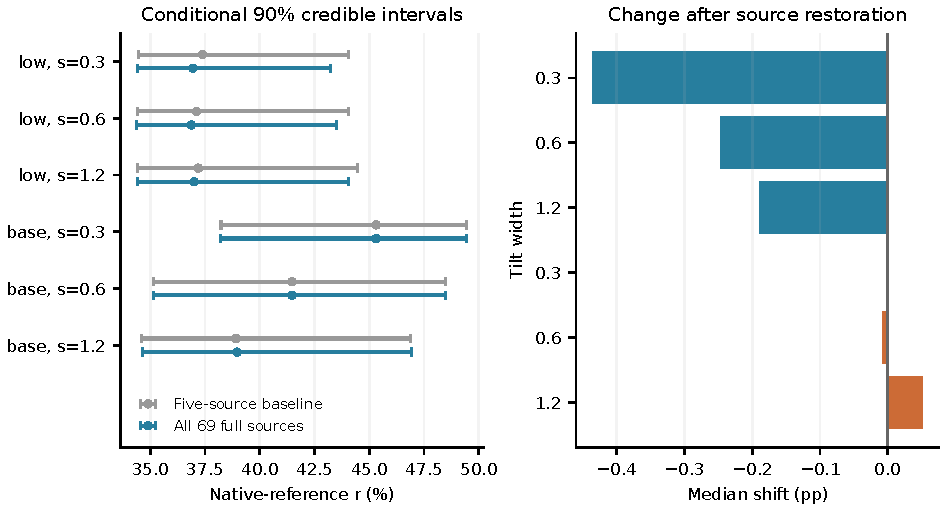
\includegraphics[width=\linewidth]{native-restoration.pdf}
\caption{全部来源恢复前后的原生参考条件诊断。左：中位数与等尾90\%可信区间。右：单独尺度上的中位数位移。“Low”“base”指固定幅度分布。这些不是共同参考倾角或渠道比例。}\label{fig:native}
\end{figure}

另一个$g$控制的匹配滤波后验摘要见表\ref{tab:g}。同一$\lambda$下的幅度族中位数差为12.10、12.89、14.34 pp，区间明显重叠。这些差异不说明两个总体统计不相容，也没有通过证据比较偏好其中某模型。去掉选择修正仅作为诊断，不是合法观测模型；其使中位数降低5.20--13.86 pp。O3并集中加入cWB则使中位数移动$-0.042$至$-0.309$ pp。这些比较轴不能合并为一条误差估计。

\begin{table}[tbp]\centering
\caption{条件$g$后验。括号是各指定模型内部的等尾90\%天体物理可信区间，与下文人工抽稀范围不同。}\label{tab:g}
\begin{tabular}{lrr}
\toprule
幅度先验 & $\lambda$ & $g$ 中位数[5\%,95\%分位数]（\%） \\
\midrule
$\mathrm{Beta}(1.5,8.5)$ & 0 & 13.29 [1.69, 32.27] \\
$\mathrm{Beta}(1.5,8.5)$ & 4 & 13.57 [1.77, 32.57] \\
$\mathrm{Beta}(1.5,8.5)$ & 16 & 14.32 [2.00, 33.33] \\
$\mathrm{Beta}(2,5)$ & 0 & 25.39 [9.26, 43.27] \\
$\mathrm{Beta}(2,5)$ & 4 & 26.47 [10.24, 44.20] \\
$\mathrm{Beta}(2,5)$ & 16 & 28.66 [12.33, 46.06] \\
\bottomrule
\end{tabular}

\end{table}
\begin{figure}[tbp]\centering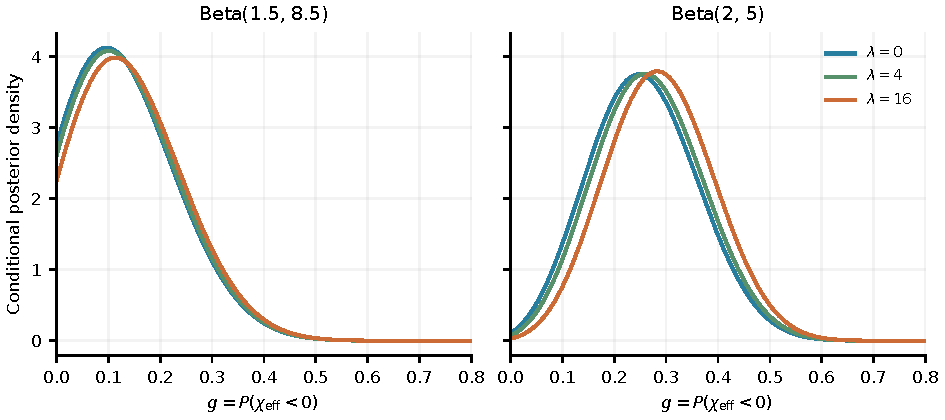
\includegraphics[width=\linewidth]{effective-spin.pdf}
\caption{两幅度族在相同均匀$g$先验下的条件后验密度。选择处理、事件集与质量/红移因子固定。图示到$g=0.8$，归一化与全部计算均使用$[0,1]$。}\label{fig:g}
\end{figure}

\subsection{分析标签的反例}
GW190421\_213856的Phenom与Mixed在完整双射连接后，包含相同的147,856个原生后验点，但派生的主黑洞无穷远倾角余弦最大相差0.12980。Phenom配置明确为16 Hz；Mixed缺少对应参考元数据。记录的PESummary版本对应到一段历史源码：参考缺失时补20 Hz。独立数值控制将两套派生字段分别与16、20 Hz联系起来。因此原生样本相同，不保证参考依赖的派生列相同。

先用20行诊断，再用另外70条留出/压力行验证。一条$1.2323\times10^{-6}$残差超过原定$10^{-6}$发布值一致性门槛。两求解器的更严积分彼此一致，却未消除该差异。在同一70行上重放未经改写的历史LALSuite 7.0 Python默认例程，可分别在$3.87\times10^{-8}$与$4.43\times10^{-8}$内复现发布值，支持历史默认数值精度的解释。该跟进在看到失败后复用原行，不是新留出测试。原门槛仍标为失败，也没有重建完整历史运行环境。

\begin{figure}[tbp]\centering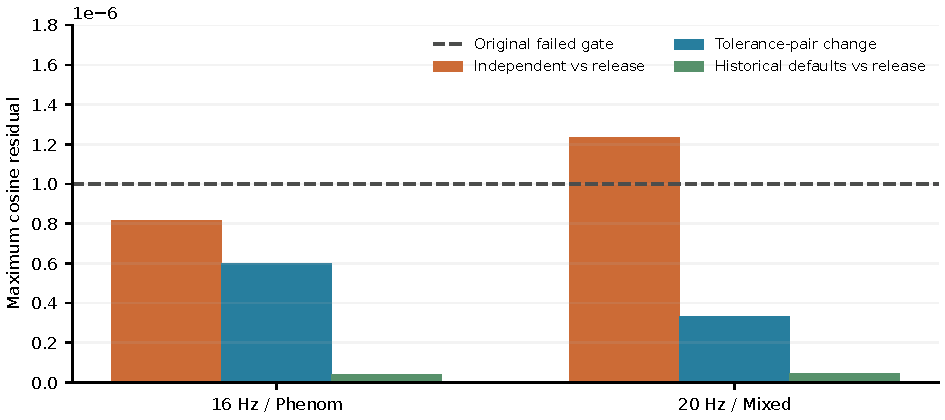
\includegraphics[width=\linewidth]{reference-residual.pdf}
\caption{原发布值一致性失败保留。历史默认值重放在固定70行上解释了小残差，不将独立求解器原测试重新标为通过。}\label{fig:reference}
\end{figure}

\FloatBarrier
\section{成对有限银行实验}\label{sec:banks}
\subsection{设计与协方差}
设计在这些抽稀输出前记录。每次从各事件完整银行无放回等概率抽取\DataEventDraw{}行，共\DataReplicates{}次；另独立从O3接受银行\DataOThreeRows{}行抽取\DataOThreeDraw{}行。观测数始终为\DataEvents{}，O1/O2贡献固定。共享索引同时配对两个指标、六模型和两搜索规则。事件流使用种子序列$[20261026,\mathrm{source\ index}]$，O3种子为20261025。沿用旧O3随机流是成对重分析，不是新增独立重复。事件抽稀不复现历史宇宙学先验拒绝抽样。

银行大小为$M$、保留数为$n$、行向量权重为$w_j$时，该指定有限总体设计满足
\begin{equation}
 \operatorname{Cov}(\bar w_n)=\frac{1-n/M}{n}\,
 \frac{1}{M-1}\sum_{j=1}^M(w_j-\bar w_M)(w_j-\bar w_M)^T.\label{eq:cov}
\end{equation}
事件向量含两个指标和六组分量对，共24维；O3向量还联合覆盖两搜索规则。搜索未通过的接受行在抽样框中保持零权重。以Jacobian传播联合协方差，同时另行计算完整非线性后验。共享配对保留独立误差棒无法表达的抵消和交互。

\subsection{结果与核查}
表\ref{tab:finite}和图\ref{fig:finite}总结该设计。接近零的原生低自旋宽度差，在\DataOThreeLowNonpositive\%的仅O3抽稀和\DataJointLowNonpositive\%的联合抽稀中非正。这些是人工重复的条件频率，不是$p$值。相应仅事件、仅O3、联合标准差为0.17642、0.49261、0.56206 pp。显式非线性交互
\begin{equation}
 \Delta_{\rm int}=T_{\rm joint}-T_{\rm event}-T_{\rm O3}+T_{\rm full}
\end{equation}
的RMS为\DataInteraction{} pp。只用线性方差不能复现每项小差异。有效自旋的三项幅度差在全部512次联合重复中为正；该结论仅针对指定银行与抽样数。

\begin{table}[tbp]\centering\small
\caption{中位数差，单位pp。原生$\Delta r$为$\sigma=0.3$减1.2，$\Delta g$为Beta(2,5)减Beta(1.5,8.5)。括号是指定人工抽稀的5\%--95\%分位范围，不是可信区间、置信区间或真实活动误差。}\label{tab:finite}
\begin{tabular}{lrrrr}
\toprule
对比 & 全银行 & 仅事件 & 仅O3 & 联合 \\
\midrule
$\Delta r$，低自旋 & -0.060 & [-0.278, 0.289] & [-0.676, 0.932] & [-0.661, 1.075] \\
$\Delta r$，基线幅度 & 6.354 & [6.112, 6.637] & [5.548, 7.052] & [5.564, 7.096] \\
$\Delta g$，$\lambda=0$ & 12.098 & [10.412, 13.225] & [9.792, 14.164] & [9.097, 14.333] \\
$\Delta g$，$\lambda=4$ & 12.892 & [11.193, 14.041] & [10.546, 15.001] & [9.871, 15.135] \\
$\Delta g$，$\lambda=16$ & 14.342 & [12.598, 15.522] & [11.874, 16.570] & [11.122, 16.724] \\
\bottomrule
\end{tabular}

\end{table}
\begin{figure}[tbp]\centering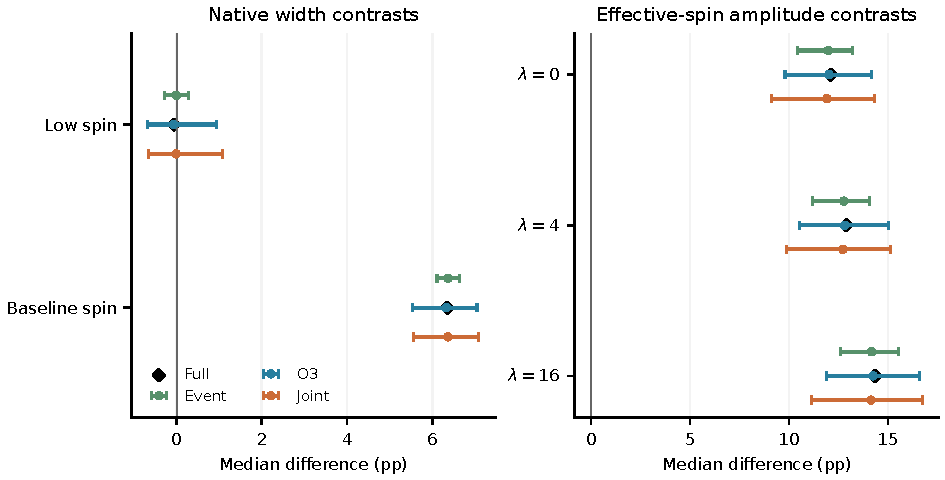
\includegraphics[width=\linewidth]{finite-banks.pdf}
\caption{人工抽稀的中位数差。线为5\%--95\%分位范围，圆点为重复中位数，黑菱形使用完整银行。全程固定O1/O2和相同69个观测。}\label{fig:finite}
\end{figure}

独立事件验证器重算源坐标均值、全部69个有限银行协方差，核验每源512组索引流指纹，并在选定重复上直接核查抽样和，选点包括每项对比的极值。全部512次仅事件和联合后验均以完整乘积核查，最大分位数差分别为$1.53\times10^{-14}$、$1.40\times10^{-14}$。这不表示每次重复中的全部抽样权重和都已独立逐行重算。

另一项保留的数值失败涉及弱导数。$10^{-6}$实相对步长给出最大相对差$1.04060\times10^{-4}$，超过不变的$10^{-4}$门槛；相关中位数差只有约$6\times10^{-12}$，容易受消减误差影响。$10^{-5}$步长在原门槛下通过，最大误差$4.88\times10^{-6}$；两种步长的固定插值区间复数微分独立核查到$9.51\times10^{-11}$。生产后验、抽样和解析Jacobian没有修改，原步长仍记为失败。

\section{银行无法揭示的贡献}\label{sec:support}
\subsection{条件后验包络界}
设$p(g)$为基线后验，修正后验正比于$p(g)h(g)$，且$h>0$。假设
\begin{equation}
 \operatorname*{ess\,sup}_g\log h(g)-\operatorname*{ess\,inf}_g\log h(g)\leq B,\label{eq:B}
\end{equation}
但不声称数据已建立这一上界。$h$中的任意常数会抵消，因而可令$1\leq h\leq R=e^B$。任意阈值下基线累计概率为$F$时，阈值下权重取一、阈值上取$R$，得到最小修正累计质量；反过来得到最大值。因此
\begin{equation}
 \frac{F}{F+e^B(1-F)}\leq F_h\leq\frac{e^BF}{1-F+e^BF}.\label{eq:cdf}
\end{equation}
记$s(t)=(1+e^{-t})^{-1}$，$Q$为基线分位函数，则
\begin{equation}
 Q\!\left[s(\operatorname{logit}q-B)\right]\leq Q_h(q)
 \leq Q\!\left[s(\operatorname{logit}q+B)\right].\label{eq:quantile}
\end{equation}
在满足式\eqref{eq:B}的任意正重加权函数类中，这些界是尖锐的。再对两域权重引起的概率位移取最大值，得到
\begin{equation}
 \operatorname{TV}(p_h,p)\leq\tanh(B/4).
\end{equation}
在这一宽泛数学类中达到边界，不证明同一个物理波形似然或六模型共享的检出律能够实现这些极端权重。

如果已表示积分精确，每事件遗漏贡献的均匀相对上界为$\epsilon_i$，而选择遗漏相对上界在所有$g$上为$\eta_{\rm sel}$，则一个充分预算是
\begin{equation}
 B=\sum_{i=1}^{69}\log(1+\epsilon_i)+69\log(1+\eta_{\rm sel}).\label{eq:budget}
\end{equation}
重采样和ESS都不能测出这些界。保留积分为零但补入为正时，有限均匀相对界失效。银行内MC波动是另一误差来源，没有被默认纳入式\eqref{eq:budget}。

对两个幅度模型，将基线幅度族的中位数下包络减去低幅度族的中位数上包络，可得保守差异下界。表\ref{tab:support}给出该充分排序保证触零的$B_*$。只考虑选择遗漏时，匹配滤波阈值对应1.346\%--1.598\%的均匀相对界；若仅考虑69事件等额遗漏界，也有相同换算。两类来源不能各自使用完整预算。充分排序保证失效，不代表观测到了物理翻转。

\begin{table}[tbp]\centering
\caption{条件排序保证阈值。末列为匹配滤波口径的$100[\exp(B_*/69)-1]$，对应正文一种单来源预算解释。这里没有估计实际缺失贡献界。}\label{tab:support}
\begin{tabular}{rrrr}
\toprule
$\lambda$ & $B_*$ 匹配滤波 & $B_*$ 含cWB & 等效上界（\%） \\
\midrule
0 & 0.92251 & 0.90978 & 1.346 \\
4 & 0.98246 & 0.96835 & 1.434 \\
16 & 1.09371 & 1.07682 & 1.598 \\
\bottomrule
\end{tabular}

\end{table}
\begin{figure}[tbp]\centering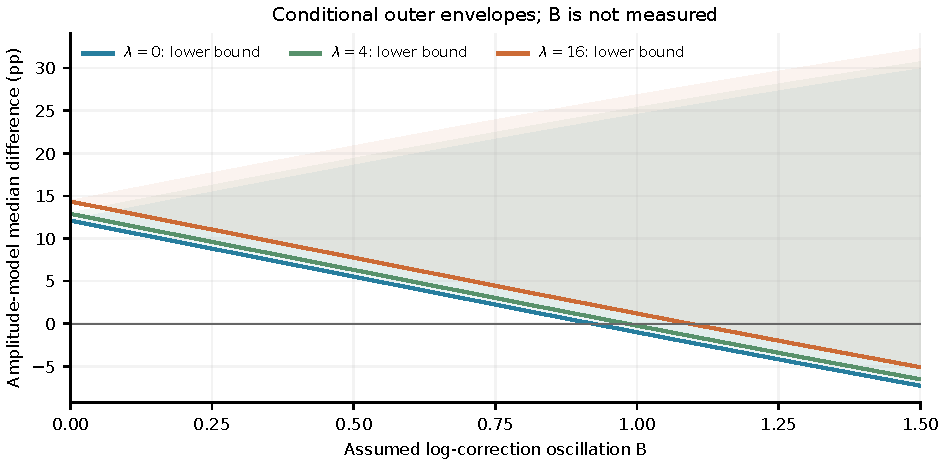
\includegraphics[width=\linewidth]{support-envelope.pdf}
\caption{幅度模型中位数差的外包络：允许每模型有满足同一假设$B$的未知修正。阴影是敏感性包络，不是可信区间；基线后验仍保留各自模型假设。}\label{fig:support}
\end{figure}

\subsection{零分量的补入族}
GW191204\_171526的\DataEventZeroRows{}条发布行，在六个$g$模型上均为零负分量权重。有限银行抽样协方差无法产生未见的负贡献。这不证明其物理负自旋似然为零。

作为诊断后声明的压力族，只将该事件的$(0,\mu_+)$改为$(\eta\mu_+,\mu_+)$，其余68事件与选择函数不变。为展示效应，六模型共用同一$\eta$；它是积分比，不是缺失后验概率，也不是拟合参数。归一化的$\eta\to\infty$极限仅保留负分量。匹配滤波响应见表\ref{tab:completion}。$\eta=1$时位移为1.23--1.60 pp，极限最大值为\DataCompletionMax{} pp。相同$\eta$族内三项幅度差仍为正；该族比前述外包络允许的修正更受限制。不声称同一物理似然能产生所有积分补入。

\begin{table}[tbp]\centering
\caption{单事件补入压力，单位pp。第二列覆盖六模型的中位数位移，第三列覆盖三项相同$\lambda$幅度差。这些范围总结声明的情景，不是统计不确定度。}\label{tab:completion}
\begin{tabular}{rrr}
\toprule
$\eta$ & 六模型中位数位移范围 & 三项幅度差范围 \\
\midrule
0.0 & [-0.000, 0.000] & [12.098, 14.342] \\
0.01 & [0.014, 0.022] & [12.105, 14.350] \\
1.0 & [1.233, 1.602] & [12.439, 14.649] \\
$\infty$ & [5.201, 8.023] & [9.782, 11.682] \\
\bottomrule
\end{tabular}

\end{table}

\subsection{O3已知遗漏域与验证精度要求}
目标红移分布在$1.9<z\leq2.3$上有\DataTailMass\%的质量，超出O3提议支持。已知遗漏并集还包括任一自旋幅度超过0.998的部分；对这两个Beta族，其质量几乎完全由红移尾部主导。仅使用$P_{\rm det}\leq1$，O3时间加权遗漏贡献的上界仍约为\DataTailBound，达到基线中位数附近已表示效率的137--143倍，无法认证选择修正足够小。这只是所述遗漏域贡献的界，不是全部选择偏差的界。

连续宇宙学尾部积分与实际代码的线性插值密度分别记录。上界使用代码测度，保留极小的归一化偏差，避免将连续近似与已表示效率混用。同样，没有额外似然信息时，PE支持外很小的先验质量也不能独自约束事件似然积分。

资源计算让一种后续实验具体化。若假设均匀选择遗漏容差为0.5\%，可分别对六模型的两个符号分量，从遗漏域的目标条件分布直接独立抽样，再使用核验的历史O3并集协议评估。在零检出情形下，用精确二项上界和12分量Bonferroni控制，要达到同时95\%界，合计需\DataTailPlan{}条直接抽样。这是规划数量，不是已执行的活动；出现检出后须重算。重要性加权银行、相关抽样或新选协议不自动符合该设计。历史参考、噪声/时间平均与搜索配置必须先核验。事件遗漏和已表示银行的不确定性也仍需单独预算。

\subsection{独立支持验证}
九种补入、两搜索规则、六模型均用普通后验乘积核查。Simpson累计积分和直接分位求根与生产摘要最大相差$2.16\times10^{-7}$，通过固定$2\times10^{-6}$门槛。从两CDF之和为一的共同位置独立求$B_*$，差不超过$1.31\times10^{-6}$。分域积分核查CDF界到$2.99\times10^{-7}$，两点计算达到TV界。独立体积积分、插值测度的多项式原函数及Beta生存积分核查支持质量。这些只验证代数与实现，不验证真实$B$、$\eta$或实际覆盖率保证。

\FloatBarrier
\section{解释与尚缺的科学证据}
可以区分三个结论。第一，来源恢复会改变一项小的原生倾角排序，即使绝对中位数位移都不到半个百分点。第二，指定的有效自旋幅度差经受住了声明的成对有限银行扰动。第三，这种稳定性无法认证对未见似然和检出贡献的稳健性。支持研究给出了条件界与压力响应，没有以猜测的误差棒填补证据缺口。

模型族仍然受限：质量/红移因子固定，且自旋采用特定的条件符号/偶形状构造。未检验全部质量--自旋相关性，未对照物理形成渠道库，也未边缘化其理论不确定性。模型内可信区间重叠、中位数排序在抽稀中保持、在更宽修正类中无法保证排序，分别回答不同问题，不能单独据此建立渠道分支比例。

共同参考原生倾角、实际注入参考/执行信息、PE链相关性、共享波形系统误差与实际遗漏似然仍未校准。对更强物理解读而言，这些是实质性科学要求，不是文字上的保留。本研究也没有以新目录发布为由，将冻结GWTC-3时期数据改称全量最新推断。扩展目录需要重新核对来源、事件掩码和注入版本。

下一步应通过似然计算或核验的检出实验约束遗漏贡献，开展带理论干扰设定的物理渠道对照，并进行与完整协议匹配的恢复/覆盖率实验。改进可视化不能替代这些证据。工作台应在每项图示旁呈现指标、假设、参考约定、来源和不确定度类型。

\section{结论}
恢复全部原始先验来源并进行成对数值实验，比将预处理数组当成完整证据更能支持条件比较。小的原生倾角排序不稳定；所选有效自旋幅度差在指定人工抽稀下稳定。它们在已保存支持之外的物理稳健性仍未建立。定量边界说明需要补充哪些证据，同时保留失败检查，避免将现象学参数转换为形成渠道比例。

\appendix
\section{复现与证据入口}\label{app:repro}
代码仓库为\href{https://github.com/wkryyds4-netizen/blackhole-research-workbench}{Blackhole Research Workbench}。本稿生成时，v0.3后续研究仍在本地，尚未推送；该链接不表示当前公开HEAD已经包含这些材料。大型HDF/NPZ、环境与第三方源码快照另行获取。研究记录保存下载URL、版本与校验值；原创代码和上游材料分别遵循各自许可。

科学入口是\path{research/population-catalog/README.md}。

完整复现步骤另见\path{research/REPRODUCING_POPULATION.md}。完整来源、不变量控制、成对银行、支持与阶段JSON分别连接对应计算和独立验证器。v0.2冻结输入保留。不要执行根目录\path{model.py}，它会替换冻结产物；导入已记录函数与执行该脚本不同。\path{run_control.py}的字节参与事件积分缓存协议，修改时应版本化。

本稿的\path{research/paper/v0.3/build_evidence.py}先核验结果/验证哈希连接，再为两语言生成相同数值事实和表格，并生成出版尺寸的矢量图。随稿保存LaTeX源码、图件PDF、科学来源哈希、编译诊断、导出PDF哈希与渲染页面检查记录。重新编译可能改变PDF字节；哈希一致本身不是语义或科学验证。稿件直接以LaTeX撰写，未提交arXiv；一般源文件准备参考其说明\cite{arxivtex}。

本轮数值环境为Python 3.14.5、NumPy 2.4.6、SciPy 1.18.0、Astropy 8.0.1、Matplotlib 3.11.0。HDF提取与自旋输运采用另行记录的隔离环境。后来的累计发布与历史源码诊断，仍与正文六模型的精确输入分开。

\section*{署名与研究状态}
澄衡（Chengheng）是本项目协作AI助手（ChatGPT，OpenAI）使用的研究笔名，不表示机构背书。本稿是未经同行评审的计算研究稿；这一署名不自动满足期刊或存储库的投稿资格和作者责任要求。公开引力波数据及所引上游软件使分析得以开展。没有声称独立人类同行评审或新的物理形成渠道测量。

\begin{thebibliography}{99}
\bibitem{zevin} M. Zevin et al., One Channel to Rule Them All? Constraining the Origins of Binary Black Holes using Multiple Formation Pathways, Astrophys. J. 910, 152 (2021), \href{https://arxiv.org/abs/2011.10057v2}{arXiv:2011.10057v2}.
\bibitem{spinlike} S. Vitale, S. Biscoveanu, and C. Talbot, Spin it as you like: the (lack of a) measurement of the spin tilt distribution with LIGO-Virgo-KAGRA binary black holes, A\&A 668, L2 (2022), \href{https://arxiv.org/abs/2209.06978v3}{arXiv:2209.06978v3}.
\bibitem{infinity} M. Mould and D. Gerosa, Gravitational-wave population inference at past time infinity, Phys. Rev. D 105, 024076 (2022), \href{https://arxiv.org/abs/2110.05507v2}{arXiv:2110.05507v2}.
\bibitem{growing} C. Talbot and J. Golomb, Growing Pains: Understanding the Impact of Likelihood Uncertainty on Hierarchical Bayesian Inference for Gravitational-Wave Astronomy, MNRAS 526, 3495 (2023), \href{https://arxiv.org/html/2304.06138v2}{arXiv:2304.06138v2}.
\bibitem{structure} J. Golomb and C. Talbot, Searching for structure in the binary black hole spin distribution, Phys. Rev. D 108, 103009 (2023), \href{https://arxiv.org/html/2210.12287v2}{arXiv:2210.12287v2}.
\bibitem{injections} R. Essick et al., Compact Binary Coalescence Sensitivity Estimates with Injection Campaigns during the LIGO-Virgo-KAGRA Collaborations' Fourth Observing Run (2025), \href{https://arxiv.org/html/2508.10638v2}{arXiv:2508.10638v2}. O4 conventions in this work are not used to supply missing historical O3 execution metadata.
\bibitem{longroad} S. Vitale and M. Mould, The Long Road to Alignment: Measuring Black Hole Spin Orientation with Expanding Gravitational-Wave Datasets (2025), \href{https://arxiv.org/abs/2505.14875v2}{arXiv:2505.14875v2}.
\bibitem{degeneracies} N. E. Wolfe, A. Hussain, J. Heinzel, and S. Vitale, Binary-black hole spin population results may be driven by prior degeneracies (2026), \href{https://arxiv.org/abs/2609.10753v1}{arXiv:2609.10753v1}.
\bibitem{spinpriors} K. Kobayashi, M. Iwaya, S. Morisaki, K. Hotokezaka, and T. Kinugawa, Impact of Spin Priors on the Population Inference of Merging Binary Black Holes (2026), \href{https://arxiv.org/abs/2602.12509v2}{arXiv:2602.12509v2}.
\bibitem{tutorial} C. Talbot et al., Population inference on GWTC-3, GWPopulation example notebook, \href{https://colmtalbot.github.io/gwpopulation/examples/GWTC3.html}{tutorial}; \href{https://github.com/ColmTalbot/gwpopulation/blob/2daa71e8c56362f2f64e2166a0055478557f239a/examples/GWTC3.ipynb}{commit-pinned source}. Retrieved versions and source hashes are recorded with this project.
\bibitem{pe21} LIGO Scientific Collaboration and Virgo Collaboration, GWTC-2.1 Parameter Estimation Data Release, version v2 (2022), \href{https://zenodo.org/records/6513631}{Zenodo 6513631}. Specific original-prior files and analysis labels are identified in the source manifests.
\bibitem{pe3} LIGO Scientific Collaboration, Virgo Collaboration, and KAGRA Collaboration, GWTC-3 Parameter Estimation Data Release (2021), \href{https://zenodo.org/records/5546663}{Zenodo 5546663}. Use the fixed files/checksums in the source manifests rather than an unspecified latest version.
\bibitem{o3} LIGO Scientific Collaboration, Virgo Collaboration, and KAGRA Collaboration, O3 Search Sensitivity Estimates (2023), \href{https://zenodo.org/records/7890437}{Zenodo 7890437}; fixed file \path{endo3_bbhpop-LIGO-T2100113-v12.hdf5}.
\bibitem{lvk3} LIGO Scientific Collaboration, Virgo Collaboration, and KAGRA Collaboration, The population of merging compact binaries inferred using gravitational waves through GWTC-3, Phys. Rev. X 13, 011048 (2023), \href{https://arxiv.org/abs/2111.03634v3}{arXiv:2111.03634v3}, Appendix A.
\bibitem{arxivtex} arXiv, Submit TeX/LaTeX, \url{https://info.arxiv.org/help/submit_tex.html}, consulted 25 October 2026. This draft has not been submitted to arXiv.
\end{thebibliography}

